\section{Zielsetzung}
\label{sec:Zielsetzung}
Das Ziel des Versuches ist die fresnelschen Formeln experimentell zu bestätigen, 
indem das Verhalten von Licht beim Auftreffen auf Grenzflächen wie zum Beispiel einem Siliziumkristall 
untersucht wird. Zudem wird der Brechungsindex von Silizium und der Brewsterwinkel bestimmt. 
\section{Theorie}
\label{sec:Theorie}
Grundlage des Versuches sind die fresnelschen Formeln, welche aus der elektromagnetischen Wellentheorie hergeleitet werden können. 
Dabei werden die Annahmen getroffen, dass es sich bei den Materialien um nicht-ferromagnetische und nicht elektrisch leitende Stoffe handelt. 
Die Strahlenleistung einer Lichtwelle in Materie ist durch den Poynting-Vektor 
\begin{equation}
    \vec{S} = \vec{E} \times \vec{H} 
    \label{eqn:Poyntingvektor}
\end{equation}
gegeben. Dabei sind $\vec{E}$ die elektrische Feldstärke und $\vec{H}$ die magnetische Feldstärke. 
Der Vektor beschreibt die Strahlungsleistung pro Fläche eines elektromagnetischen Feldes. 
Der Betrag des Vektors kann durch 
\begin{equation}
    |\vec{S}| = v \cdot \varepsilon \cdot \varepsilon_0 \cdot \vec{E}²
    \label{eqn:Poyntingbetrag}
\end{equation}
dargestellt werden, unter der Annahme, dass $\vec{E}$ und $\vec{H}$ als ebene Wellen dargestellt werden können. 
$v$ ist dabei die Geschwindigkeit der Welle, $\varepsilon$ ist die relative Dielektrizitätskonstante und $\varepsilon_0$ die elektrische Feldkonstante. 
Das elektrische Feld einer Lichtwelle kann als ebene Welle der Form 
\begin{equation}
    \vec{E} = \vec{E}_e \exp{\left(\symup{i}\left(\vec{k}\cdot \vec{r} - \omega \cdot t\right)\right)}
    \label{eqn:ebene_Welle}
\end{equation}
dargestellt werden. Dabei ist $\vec{r}$ der Ortsvektor, $t$ die Zeit, $\vec{k}$ der Wellenzahlvektor, 
$\omega$ die Kreisfrequenz und $\vec{E}_e$ die Amplitude der Welle. 
Wenn diese ebene Welle aus einem Vakuum unter einem Winkel $\alpha$ auf eine Grenzfläche fällt wird ein Teil reflektiert (mit Amplitude $\vec{E}_r$)
und ein Teil dringt ins Material ein (mit Amplitude $\vec{E}_d$). Dies ist in Abbildung (\ref{fig:allgemein}) schematisch dargestellt. 
\begin{figure}
    \centering
    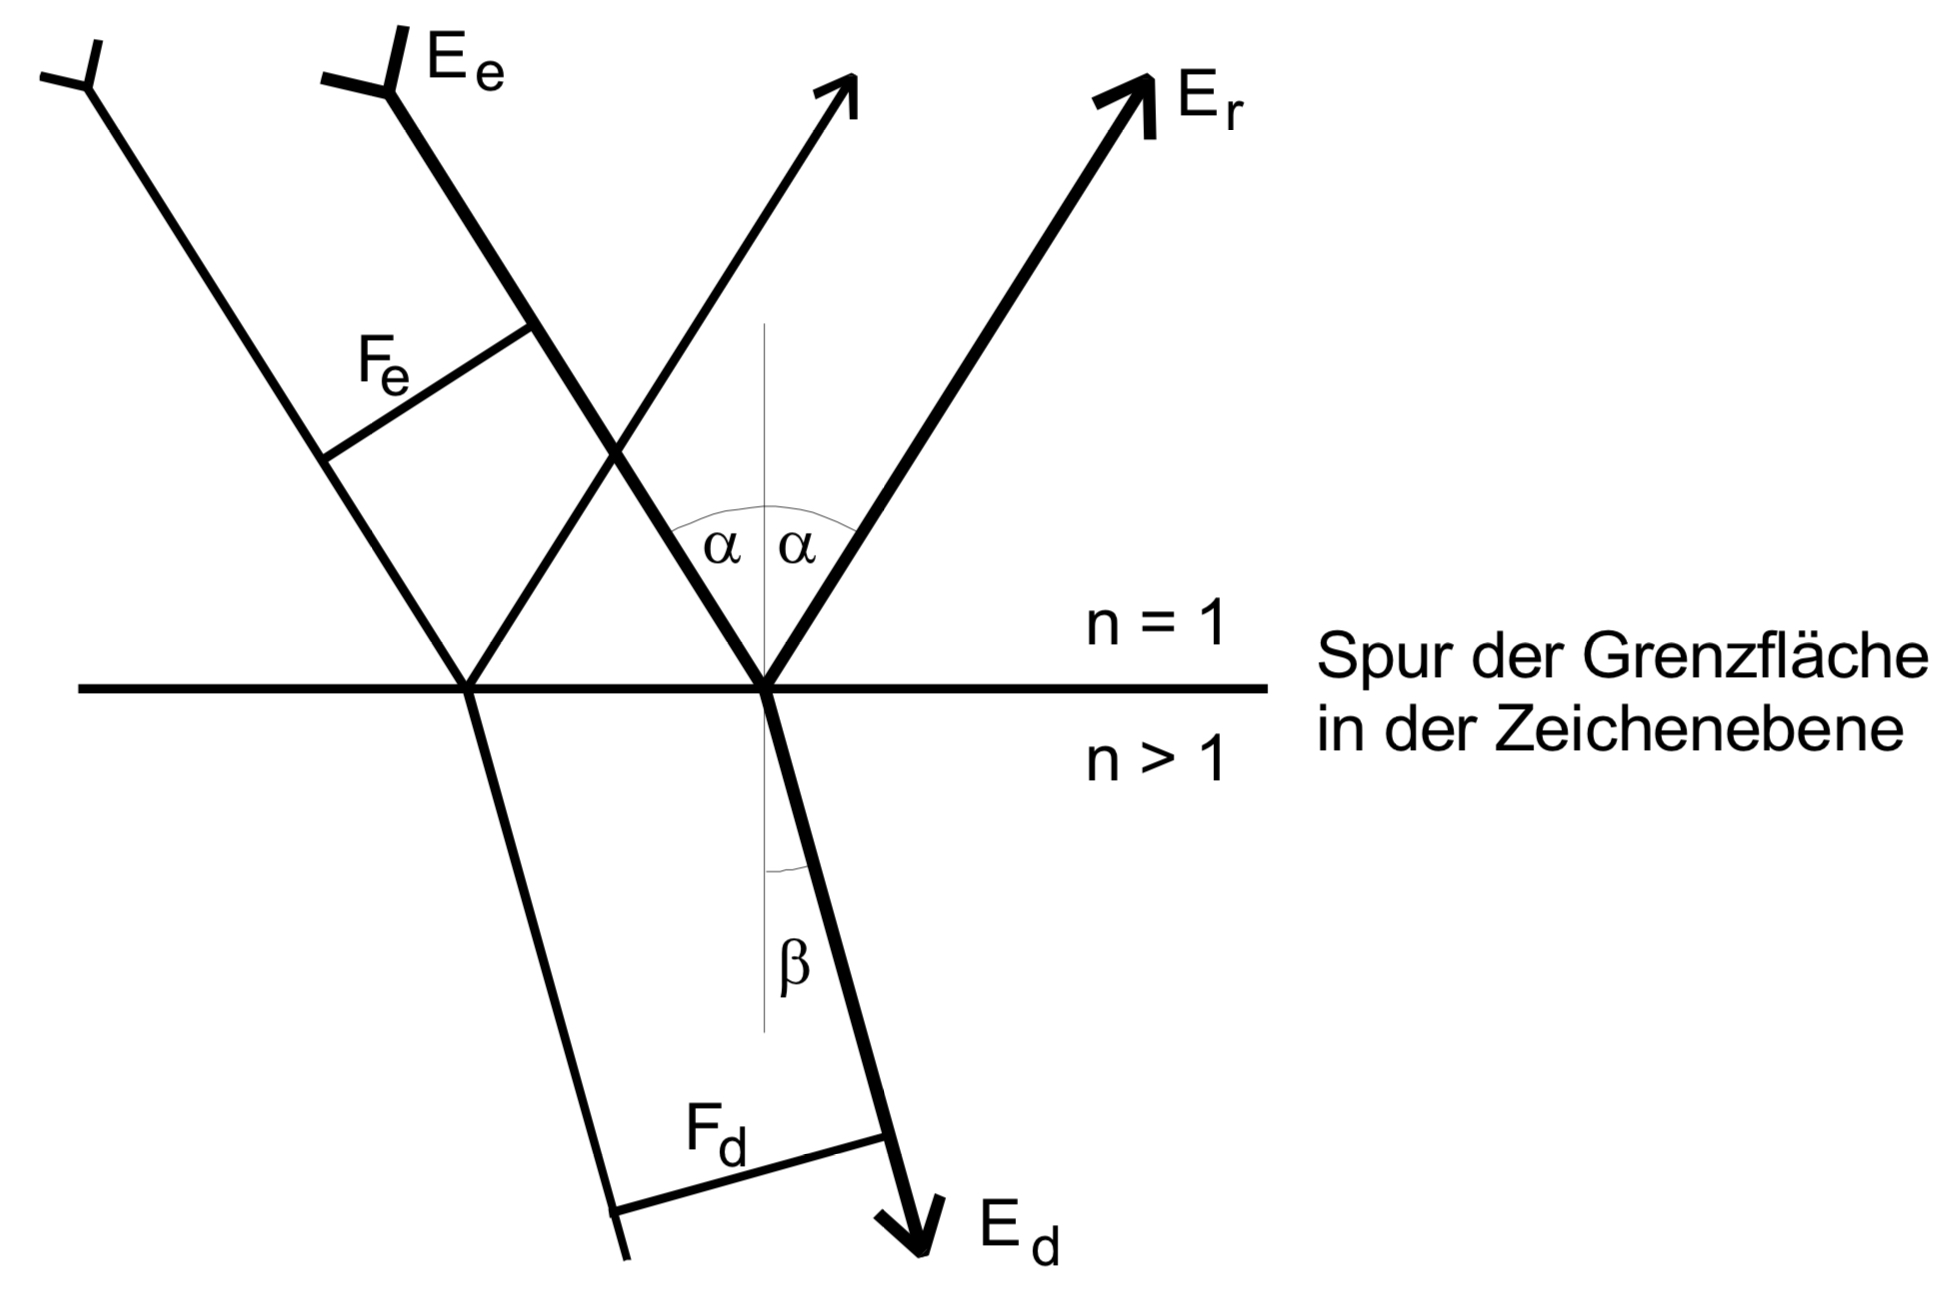
\includegraphics[width=0.65\textwidth]{content/Bilder/allgemeines_Bild.jpeg}
    \caption{Schematische Dartsellung eines auftreffenden Lichtstrahls auf eine Grenzfläche Q\cite{anleitungV407}.}
    \label{fig:allgemein}
\end{figure}
Im Material ist die Lichtgeschwindigkeit $v$ geringer als die im Vakuum $c$. Daher ändert der Lichtstrahl seine Richtung. Für Brechungsindizes 
gilt 
\begin{equation}
    n = \frac{c}{v}\, .
    \label{eqn:Brechungsindex}
\end{equation}
Für die weitere Beschreibung der Brechung ist die Unterteilung des Feldvektors in senkrecht und parallel zur Einfallsebene nötig. Es gilt 
\begin{equation}
    \vec{E}_e = \vec{E}_{\perp} + \vec{E}_{\parallel} \, .
    \label{eqn:Aufteilung}
\end{equation}
Zuerst wird die Komponente betrachtet, die senkrecht zur Einfallsebene schwingt und damit tangential zur Grenzfläche. 
Die Tangentialkomponente des Feldstärkenvektors geht stetig durch die Grenzfläche hindurch, daher gilt 
\begin{equation}
    \vec{E}_{e,\perp} + \vec{E}_{r,\perp} = \vec{E}_{d,\perp} \, .
\end{equation}
Diese Relation und das Snelliussche Brechungsgesetz 
\begin{equation}
    n = \frac{\sin{\alpha}}{\sin{\beta}}
    \label{eqn:snivellus}
\end{equation}
werden verwendet, um die Relation 
\begin{equation}
    \vec{E}_{r,\perp} = - \vec{E}_{e,\perp} \frac{\left(\sqrt{n² - \sin²{\alpha}}- \cos{\alpha}\right)}{n² - 1}
    \label{eqn:E_r_senkrecht}
\end{equation}
aufzustellen.
Für den Fall der Komponente $\vec{E}_{\parallel}$ ergibt sich 
\begin{equation}
    \vec{E}_{r,\parallel} = \vec{E}_{e,\parallel} \frac{n² \cos{\alpha} - \sqrt{n² - \sin²{\alpha}}}{n² \cos{\alpha} + \sqrt{n² - \sin²{\alpha}}} \, .
    \label{eqn:E_r_parallel}
\end{equation}
Aus der Gleichung geht hervor, dass es einen Winkel gibt unter dem keine Reflektion mehr stattfindet, sondern der Lichtstrahl ganz in das Medium eindringt. 
Dieser Winkel ist der Brewstersche Winkel $\alpha_B$. Für diesen gilt
\begin{equation}
    \tan{\alpha_B} = n \, .
    \label{eqn:Brewster}
\end{equation}
%\begin{figure}
%    \centering
%    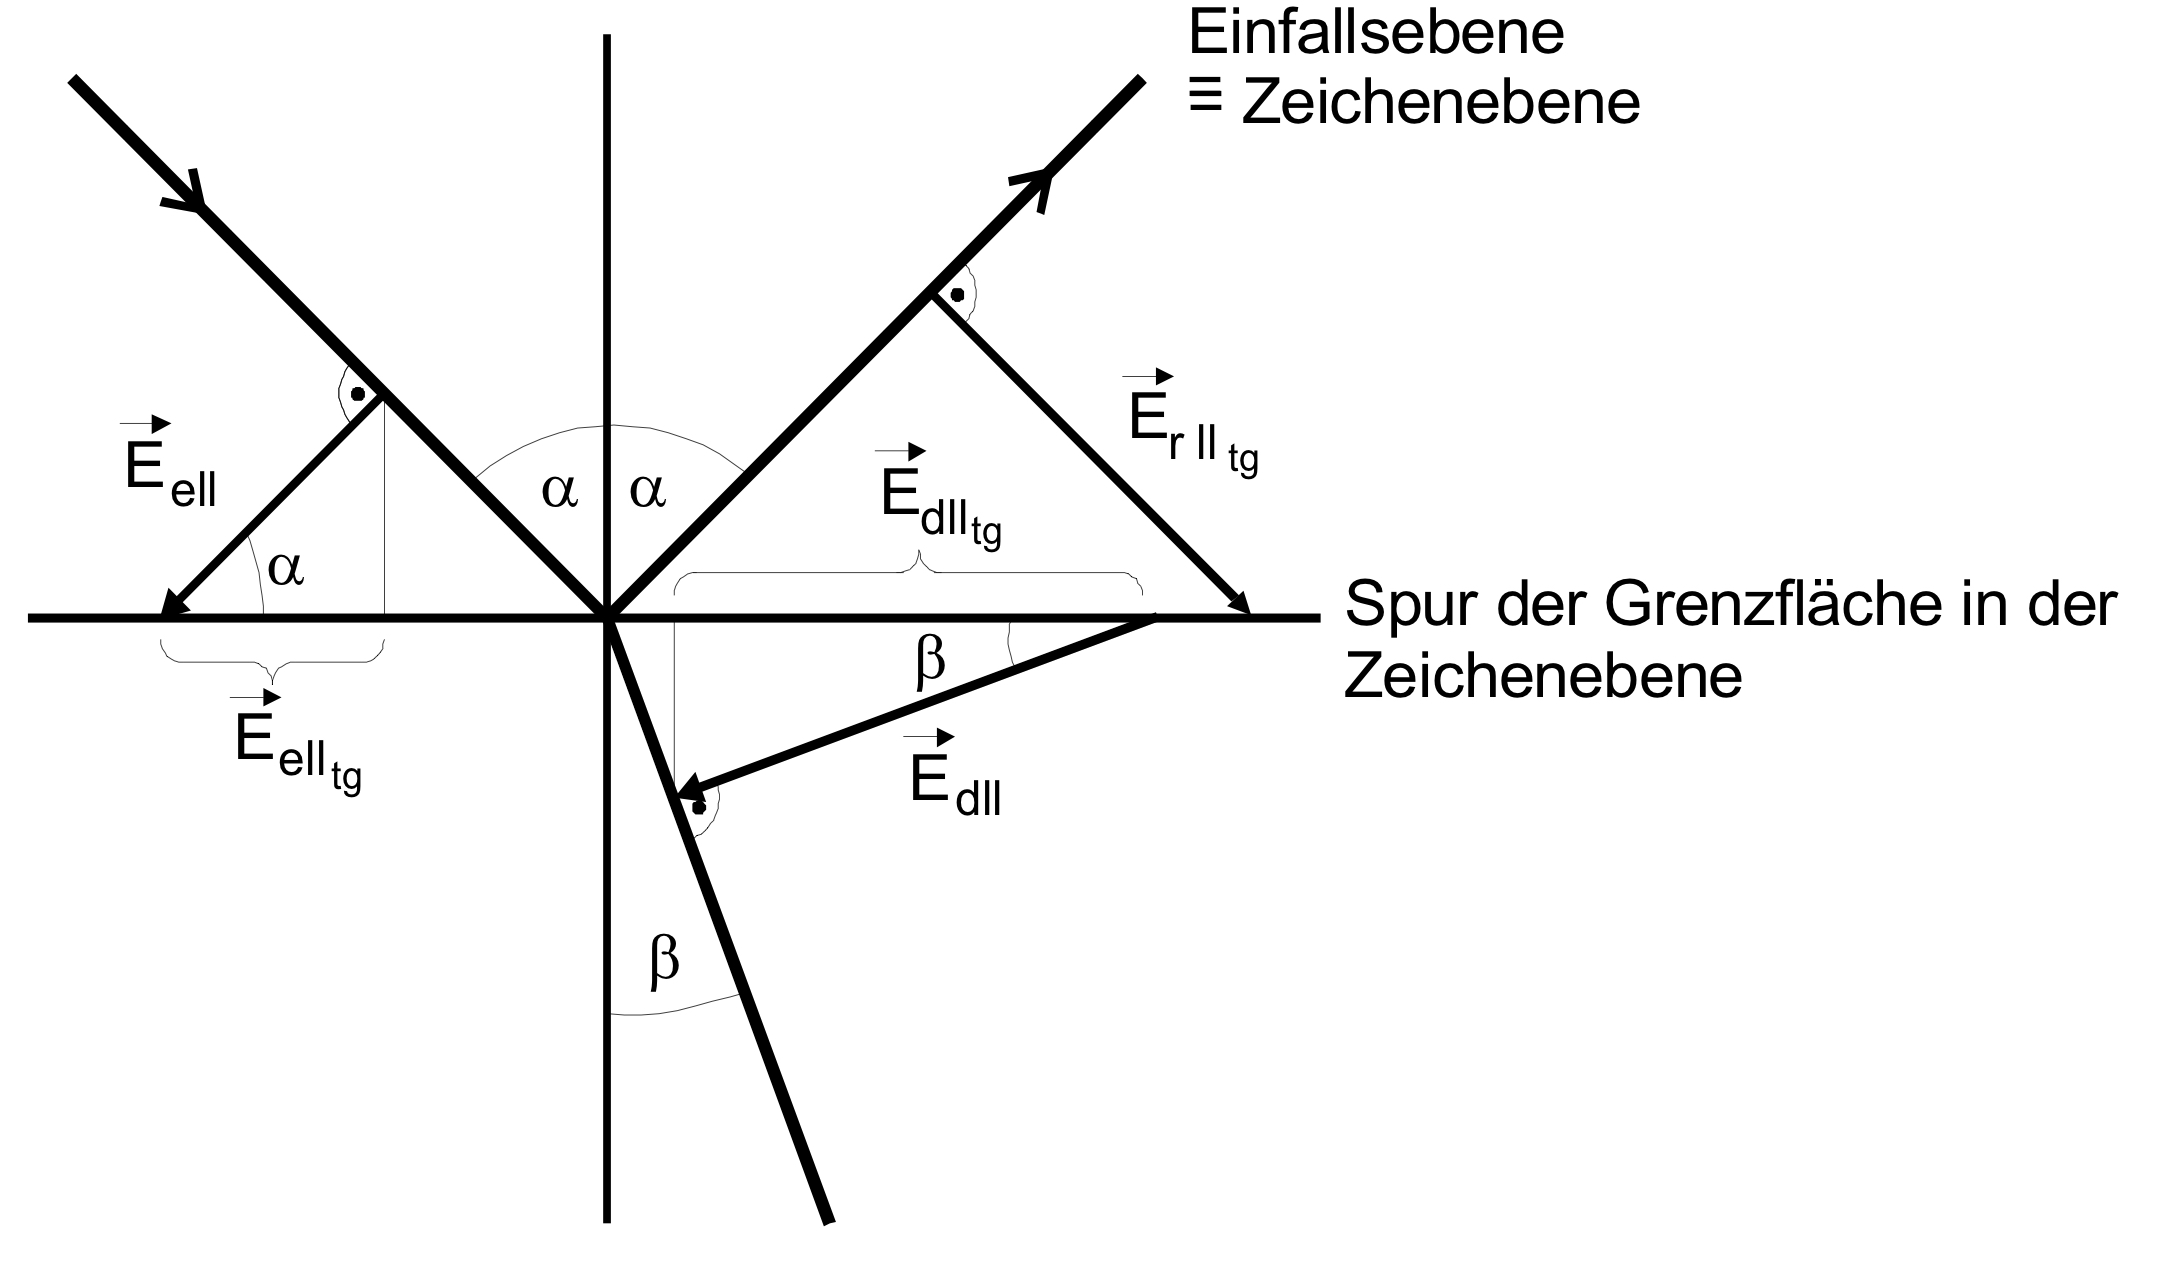
\includegraphics[width=0.65\textwidth]{content/Bilder/2.Abbildung.jpeg}
%    \caption{Schematische Darstellung eines in der Einfallebene schwindeneden Lichtstrahls. Q\cite{anleitungV407}}
%    \label{fig:2.Fall}
%\end{figure}